\subsubsection{Heurística Constructiva Golosa}

\subsubsubsection{Medición en base a tamaño del grafo}
La complejidad de la heurística constructiva golosa es $\mathcal{O}(n * (log(n) + D))$, con lo cual se espera una curva que crezca a medida que se incrementa el valor de n.

\begin{figure}[H]
	\centering
	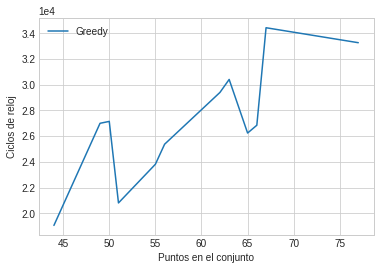
\includegraphics[scale=0.6]{exercise5/greedy3.png}
\end{figure}

El resultado obtenido es similar al esperado ya que se pueden detectar casos en los que la ejecución es más rápida que puntos anteriores. Sin embargo, la curva luego vuelve a crecer, consistentemente con nuestra suposición. 

Los casos de resoluciones rápidas podrían deberse a juegos de datos que favorecen a la heurística. Un ejemplo de esto puede ser que gran parte de las demandas sean congruentes con el stock del camión, inverso al caso ``Demandas incongruentes con el stock del camión`` explicado previamente en el desarrollo de la heurística.